\documentclass[12pt,a4paper]{article}
\usepackage{amsmath} 
\usepackage{amsfonts}
\usepackage{amssymb}
\usepackage{tikz}
\usetikzlibrary{arrows.meta, positioning, fit, backgrounds, calc}
\usepackage{graphicx}
\usepackage{tabularx} 
\usepackage[table]{xcolor} 
\usepackage{float}
\usepackage{caption} 
\usepackage[utf8]{inputenc}
\usepackage[T5]{fontenc} 
\usepackage[vietnamese]{babel}
\usepackage{geometry}
\usepackage{subcaption}
\usepackage{tikz}
\usepackage{enumitem}
\geometry{
    a4paper,
    left=30mm,
    right=20mm,
    top=20mm,
    bottom=20mm
}
\renewcommand{\arraystretch}{1.2} 
\linespread{1.2} 

\usepackage{fancyhdr}
\setlength{\headheight}{15pt}
\pagestyle{fancy}
\fancyhf{} 

% Tùy chỉnh Header
\lhead{\small \textbf{Trường Đại học Bách Khoa TP.HCM}} 
\rhead{\small Nén ảnh bằng biến đổi Haar Wavelet} 

\rfoot{\small Trang \thepage} 

% Độ dày của đường kẻ ngang
\renewcommand{\headrulewidth}{0.4pt}
\renewcommand{\footrulewidth}{0.4pt}




\usepackage{xurl}
\usepackage{hyperref}


\usepackage{listings}
\usepackage{xcolor}

% Định nghĩa các màu cơ bản cho code
\definecolor{codegreen}{rgb}{0,0.6,0}
\definecolor{codegray}{rgb}{0.5,0.5,0.5}
\definecolor{codepurple}{rgb}{0.58,0,0.82}
\definecolor{backcolour}{rgb}{0.95,0.95,0.92}

% Thiết lập style dành riêng cho code MATLAB
\lstdefinestyle{matlabstyle}{
    backgroundcolor=\color{backcolour},   
    commentstyle=\color{codegreen},
    keywordstyle=\color{blue},
    numberstyle=\tiny\color{codegray},
    stringstyle=\color{codepurple},
    basicstyle=\ttfamily\footnotesize,
    breakatwhitespace=false,         
    breaklines=true,                 
    captionpos=b,                    
    keepspaces=true,                 
    numbers=left,                    
    numbersep=5pt,                  
    showspaces=false,                
    showstringspaces=false,
    showtabs=false,                  
    tabsize=4
}
\lstset{style=matlabstyle}


\definecolor{BKB}{RGB}{0, 84, 166} 

\begin{document}

    % 1. Trang bìa 
    \begin{titlepage}
    \begin{tikzpicture}[remember picture, overlay]
        % Khung viền
        \coordinate (NW) at ($(current page.north west) + (2.5cm,-1.5cm)$);
        \coordinate (SE) at ($(current page.south east) + (-1.5cm,1.5cm)$);
        
        \draw[BKB, line width=2.5pt] (NW) rectangle (SE);
        \draw[BKB, line width=0.8pt] ($(NW) + (0.15,-0.15)$) rectangle ($(SE) + (-0.15,0.15)$);
        
        \def\side{0.6cm}
        \draw[BKB, line width=2pt] ($(NW) + (0,-\side)$) -- (NW) -- ($(NW) + (\side,0)$);
        \draw[BKB, line width=2pt] ($(NW |- SE) + (0,\side)$) -- (NW |- SE) -- ($(NW |- SE) + (\side,0)$);
        \draw[BKB, line width=2pt] ($(SE |- NW) + (-\side,0)$) -- (SE |- NW) -- ($(SE |- NW) + (0,-\side)$);
        \draw[BKB, line width=2pt] ($(SE) + (0,\side)$) -- (SE) -- ($(SE) + (-\side,0)$);
    \end{tikzpicture}
    
    \begin{center}
        {\fontsize{14}{16}\selectfont \textbf{ĐẠI HỌC QUỐC GIA TP. HỒ CHÍ MINH} \par}
        {\fontsize{14}{16}\selectfont \textbf{TRƯỜNG ĐẠI HỌC BÁCH KHOA} \par}
        {\fontsize{14}{16}\selectfont \textbf{KHOA KHOA HỌC ỨNG DỤNG} \par}
        
        \vspace{0.4cm}
        
        \ifcsname includegraphics\endcsname
            
\includegraphics[height=4cm]{logo} 
        \fi
        
        \vspace{0.4cm}
        
        % Phần Môn học, Mã môn, Học kỳ
        {\fontsize{14}{15}\selectfont \textbf{BÀI TẬP LỚN HỌC PHẦN ĐẠI SỐ TUYẾN TÍNH} \par}
        \vspace{0.4cm}
        {\fontsize{14}{15}\selectfont \textbf{ĐỀ TÀI} \par}
        
        \begin{tikzpicture}
            \draw[BKB, line width=1.5pt] (0,0) -- (16,0);
        \end{tikzpicture}
        \vspace{0.1cm}

        {\fontsize{20}{15}\selectfont \textbf{NÉN ẢNH BẰNG PHÉP BIẾN ĐỔI HAAR} \par}

        \vspace{0.2cm}
        \begin{tikzpicture}
            \draw[BKB, line width=1.5pt] (0,0) -- (16,0);
        \end{tikzpicture}
    \end{center}
    
    
    \begin{center}
        {\fontsize{14}{15}\selectfont \textbf{LỚP L09 - NHÓM 14 - HK252} \par}
        \vspace{0.2cm}
        {\fontsize{14}{15}\selectfont \textbf{NGÀY NỘP: 02/06/2026} \par}
        \vspace{0.2cm}
        {\fontsize{14}{15}\selectfont \textbf{Giảng viên hướng dẫn: ThS. Nguyễn Xuân Mỹ} \par}
    \end{center}
    
    % Danh sách thành viên
    \begin{center}
        \vspace{0.3cm}
        \renewcommand{\arraystretch}{1.2}
        \begin{tabular}{|c|c|c|c|}
            \hline
            \textbf{Sinh viên thực hiện} & \textbf{Mã số sinh viên} & \textbf{Điểm số} & \textbf{Chữ ký} \\ \hline
            Trương Đức Trọng & 2313655 &  & \\ \hline
            Trương Ngọc Hoàng & 2211124 &  & \\ \hline
            Trương Tấn Huy & 2211294 &  & \\ \hline
            Ung Thanh Hào & 2310860 &  & \\ \hline
            Văn Thị Thu Nhung & 2014041 &  & \\ \hline
            Võ Công Chí Bảo & 2410310 &  & \\ \hline
            Võ Huỳnh Anh Thư & 2213416 &  & \\ \hline
            Võ Lê Phúc Thịnh & 2510382 &  & \\ \hline
            Võ Ngô Ngọc Thạnh & 2511550 &  & \\ \hline
            Võ Thành Tài & 2213006 &  & \\ \hline
        \end{tabular}
    \end{center}

    \vfill 
    
    \begin{center}
        {\fontsize{13}{15}\selectfont \textit{Thành phố Hồ Chí Minh - 2026}}
    \end{center}

\end{titlepage}

    \newpage
    
    % 2. Mục lục
    \pagenumbering{roman} 
    \tableofcontents
    \newpage

    % 3. Nội dung chính (Được chia theo 5 chương đã thống nhất)
    \pagenumbering{arabic}
    \setcounter{page}{1}
    \section*{LỜI CẢM ƠN}
\addcontentsline{toc}{section}{LỜI CẢM ƠN}

Lời đầu tiên, nhóm chúng em xin gửi lời cảm ơn chân thành và sâu sắc nhất đến 
cô Th.S Nguyễn Xuân Mỹ. Trong suốt thời gian học tập và nghiên cứu môn 
Đại số tuyến tính, nhờ có sự giảng dạy tận tình, tâm huyết 
và những kiến thức nền tảng vững chắc mà cô truyền đạt, 
chúng em mới có đủ cơ sở để thực hiện bài báo cáo này.
Đặc biệt, chúng em xin trân trọng cảm ơn cô đã trực tiếp hướng dẫn, 
định hướng và tạo mọi điều kiện thuận lợi giúp nhóm hoàn thành tốt đề tài 
"Nén ảnh bằng phép biến đổi Haar". Quá trình làm bài đã giúp chúng em 
không chỉ hiểu sâu hơn về lý thuyết toán học mà còn 
biết cách ứng dụng vào thực tiễn một cách sinh động.
Mặc dù cả nhóm đã nỗ lực hết sức trong quá trình nghiên cứu, 
tìm tòi và chạy thử nghiệm trên phần mềm, 
nhưng do thời gian và giới hạn kiến thức của bản thân 
nên bài tiểu luận chắc chắn vẫn còn những thiếu sót. 
Chúng em rất mong nhận được những lời nhận xét, 
góp ý và chỉ bảo quý báu từ cô để bài làm được hoàn thiện hơn, 
đồng thời giúp chúng em đúc kết thêm kinh nghiệm cho những môn học sau này.
Chúng em xin chân thành cảm ơn cô.

    \newpage

    \section*{PHẦN MỞ ĐẦU}
\addcontentsline{toc}{section}{PHẦN MỞ ĐẦU}

\subsection*{1. Đặt vấn đề thực tế}
Toán học luôn hiện hữu trong mọi mặt của cuộc sống từ những việc đơn giản nhất như tính toán số tiền phải chi trả hàng tháng cho đến áp dụng những
phương trình và phép tính phức tạp nhằm phân tích tín hiệu dùng trong truyền thông và xử lý thông tin. 
Trong kỷ nguyên số, chúng ta luôn có nhu cầu lưu giữ những khoảng khắc bằng hình ảnh và video, hoặc đăng tải và chia sẻ lên các trang mạng xã hội. 
Lượng nội dung đa phương tiện khổng lồ này đặt ra một thách thức lớn về mặt băng thông mạng và dung lượng lưu trữ. 
Đề tài nén ảnh bằng phép biến đổi Haar cho phép chúng ta có một cái nhìn sâu hơn về cách truyền tải hoặc lưu trữ một hình ảnh với dung lượng lớn mà
không vượt quá giới hạn vật lý của đường truyền.

Để hiểu rõ hơn về cách một thuật toán nén ảnh hoạt động, hãy tìm hiểu một số ví dụ về cách não bộ chúng ta xử lý nội dung
của một thông tin bất kỳ.

\textbf{Ví dụ 1 (Sự chọn lọc thông tin): }Trong đời sống hàng ngày, bất kỳ ai cũng từng phải đi chợ và lựa chọn xem hôm nay phải ăn gì.
Có những người sẽ lựa chọn thực phẩm dựa trên lượng đạm, xơ và tinh bột cần thiết cho một ngày (đó là những thông tin chung).
Tuy nhiên sẽ có những người lựa chọn kỹ hơn bằng việc xem xét thêm các yếu tố dinh dưỡng khác của thực phẩm như lượng khoáng chất, các loại vitamin (đây là những thông tin chi tiết).

\textbf{Ví dụ 2 (Sự truyền tải lần lượt):} Giả sử bạn đang tò mò muốn biết người bạn của mình đang xem bức ảnh về ai. 
\begin{itemize}
    \item Bạn hỏi: \textit{"Cậu đang xem gì thế?"} $\rightarrow$ Người bạn đáp: \textit{"Một người rất nổi tiếng."} (thông tin khái quát).
    \item Bạn nhìn kỹ hơn: \textit{"Tớ thấy rồi nhưng là ai vậy?"} $\rightarrow$ Người bạn nói thêm: \textit{"Người này là phụ nữ."} (thêm chi tiết).
    \item Bạn mất kiên nhẫn: \textit{"Cậu nói rõ hơn đi?"} $\rightarrow$ Người bạn trả lời: \textit{"Cô ấy là diễn viên Kim Ji Won"} (thông tin hoàn chỉnh).
\end{itemize}

Điểm chung của các ví dụ trên là việc thông tin có thể được chia thành nhiều mức độ chi tiết. Trong ví dụ 2, ta cũng có thể hình dung việc truyền một
hình ảnh từ máy chủ đến điện thoại người dùng theo từng bước từ ảnh mờ đến ảnh sắc nét và nhiều chi tiết. 

\begin{figure}[H]
    \centering
    % Ảnh 1
    \begin{subfigure}[b]{0.24\textwidth}
        \centering
        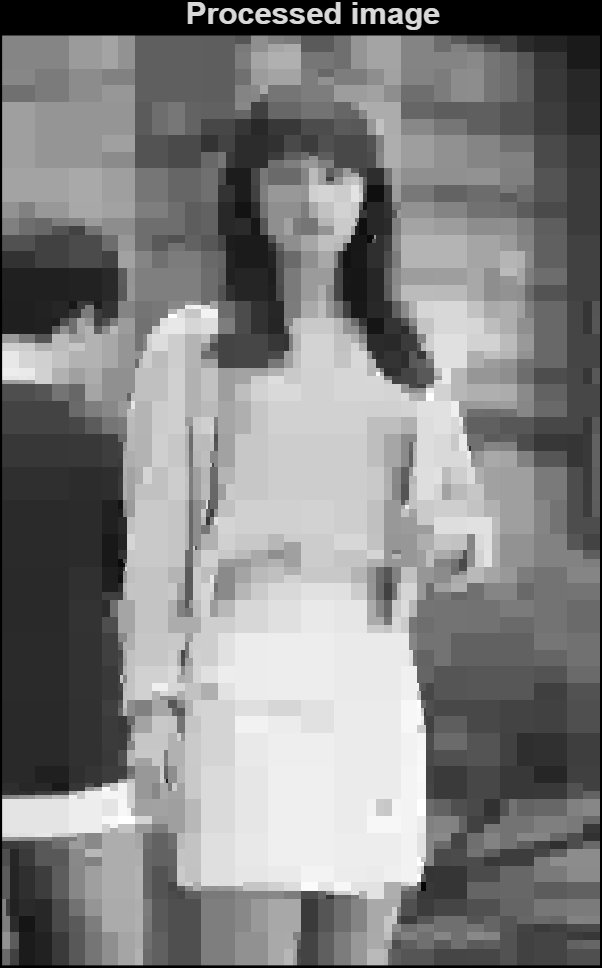
\includegraphics[width=\textwidth]{kjw1.png}
        \caption*{Người nổi tiếng}
    \end{subfigure}
    \hfill
    % Ảnh 2
    \begin{subfigure}[b]{0.24\textwidth}
        \centering
        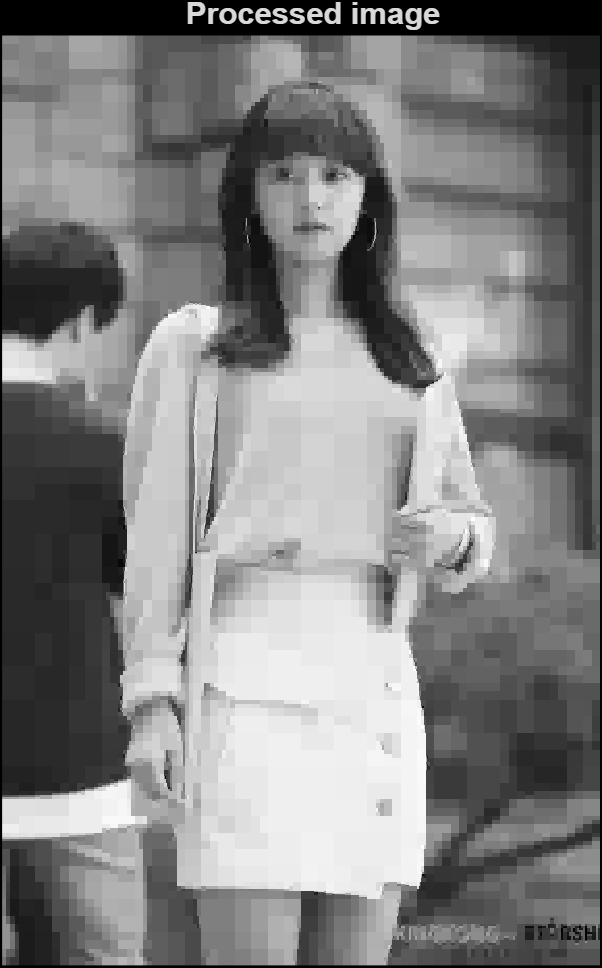
\includegraphics[width=\textwidth]{kjw2.png}
        \caption*{Người phụ nữ}
    \end{subfigure}
    \hfill
    % Ảnh 3
    \begin{subfigure}[b]{0.24\textwidth}
        \centering
        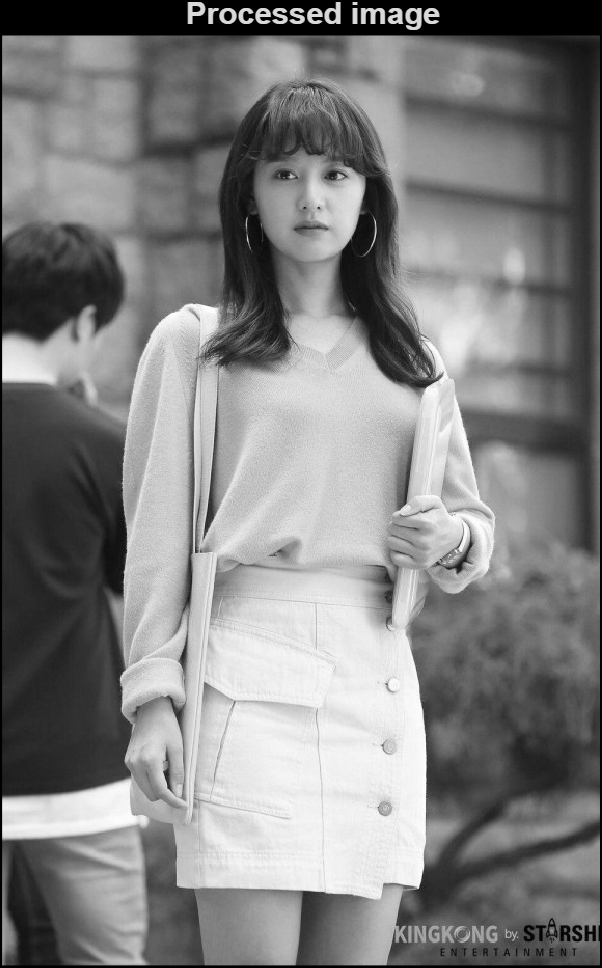
\includegraphics[width=\textwidth]{kjw3.png}
        \caption*{Diễn viên Kim Ji Won}
    \end{subfigure}
    \hfill

    \caption{Quá trình truyền tải hình ảnh.}
\end{figure}

\subsection*{2. Đối tượng và mục tiêu đề tài}

\textbf{Đối tượng nghiên cứu: } Đối tượng nghiên cứu của đề tài là phép biến đổi Haar (Haar Wavelet). Phép biến đổi sử dụng các ma trận trực giao để phân tích bức ảnh
thành các dải tần số thấp (chi tiết xấp xỉ) và các dải tần số cao (chi tiết độ nét, góc cạnh). Việc giữ lại phần xấp xỉ tổng thể và triệt tiêu một số chi tiết ta có thể thực hiện
nén một bức ảnh với dung lượng nhỏ hơn mà không gây ảnh hưởng quá nhiều đến chất lượng ảnh.

\vspace{0.3cm}
\noindent \textbf{Mục tiêu của đề tài bao gồm:}
\begin{itemize}
    \item Phân tích cơ sở lý thuyết đằng sau phép biến đổi Haar về mặt Đại số tuyến tính.
    \item Thực hiện quá trình nén ảnh và cắt ngưỡng (triệt tiêu một số chi tiết).
    \item Đánh giá hiệu năng và mức độ khôi phục hình ảnh của thuật toán.
\end{itemize}
    \newpage

    \section*{Chương 1: Cơ sở lý thuyết về biến đổi Haar Wavelet}
\addcontentsline{toc}{section}{Chương 1: Cơ sở lý thuyết về biến đổi Haar Wavelet}

\subsection*{1. Tổng quan về phép biến đổi Wavelet và Haar Wavelet}
Wavelet trong tiếng Pháp còn được hiểu là sóng con. Trong toán học, Wavelet đại diện cho những hàm sóng
có thể được co dãn và tịnh tiến. Một biến đổi Wavelet có thể biến bất kỳ tín hiệu nào thành các tín hiệu được xây dựng
từ các sóng con này.

Alfred Haar (1885-1933) là nhà toán học người Hungary, người đã giới thiệu biến đổi Haar Wavelet vào năm 1909. 
Đây là loại Wavelet đơn giản nhất, không có sự chồng chéo, chia tín hiệu thành các cặp giá trị rời rạc và xử lý cục bộ.

Biến đổi Haar Wavelet hoạt động bằng cách phân tách tín hiệu rời rạc thành hai phần có độ dài bằng nhau: 
thành phần trung bình (average) giữ lại cấu trúc tổng thể và thành phần sai khác (difference) lưu giữ những chi tiết sắc nét.
Đặc biệt hơn từ hai thành phần này ta có thể khôi phục lại được tín hiệu ban đầu một cách vô cùng chính xác. 

\subsection*{2. Phép biến đổi Haar 1D}
Để xem việc phân tích một tín hiệu bằng cách tính trung bình và sai khác như thế nào ta có thể xét một đoạn tín hiệu như sau:
$$X_{0}=(154, 150, 156, 152, 160, 160, 152, 156)^T$$
Ta chia đoạn tín hiệu trên thành từng cặp và tìm nửa tổng, nửa hiệu của các cặp đó. Ta sẽ thu được một dãy sau:
$$X_{1}=(152, 154, 160, 154, 2, 2, 0, -2)$$
Trong dãy $X_{1}$ trên, bốn số đầu tiên là nửa tổng của bốn cặp, bốn số tiếp theo là nửa hiệu của bốn cặp.
Ta có thể dùng ma trận để mô tả quá trình này như sau:
\begin{center}
    $$A = \begin{pmatrix}
        \frac{1}{2} &  \frac{1}{2} &  0 &  0 &  0 &  0 &  0 &  0 \\
        0 &  0 &  \frac{1}{2} &  \frac{1}{2} &  0 &  0 &  0 &  0 \\
        0 &  0 &  0 &  0 &  \frac{1}{2} &  \frac{1}{2} &  0 &  0 \\
        0 &  0 &  0 &  0 &  0 &  0 &  \frac{1}{2} &  \frac{1}{2} \\
        \frac{1}{2} & -\frac{1}{2} &  0 &  0 &  0 &  0 &  0 &  0 \\
        0 &  0 &  \frac{1}{2} & -\frac{1}{2} &  0 &  0 &  0 &  0 \\
        0 &  0 &  0 &  0 &  \frac{1}{2} & -\frac{1}{2} &  0 &  0 \\
        0 &  0 &  0 &  0 &  0 &  0 &  \frac{1}{2} & -\frac{1}{2}
    \end{pmatrix}$$
\end{center}

Ta thấy rằng nếu lấy tích vô hướng của từng hàng với nhau kết quả đều là 0, điều này cho thấy các hàng của ma trận $A$ tạo nên họ trực giao.
Nếu ta chia mỗi hàng cho độ dài của chúng ta được họ trực chuẩn, ma trận trực giao $H$ tương ứng như sau:
\begin{center}
    $$H = \begin{pmatrix}
        \frac{\sqrt{2}}{2} &  \frac{\sqrt{2}}{2} &  0 &  0 &  0 &  0 &  0 &  0 \\
        0 &  0 &  \frac{\sqrt{2}}{2} &  \frac{\sqrt{2}}{2} &  0 &  0 &  0 &  0 \\
        0 &  0 &  0 &  0 &  \frac{\sqrt{2}}{2} &  \frac{\sqrt{2}}{2} &  0 &  0 \\
        0 &  0 &  0 &  0 &  0 &  0 &  \frac{\sqrt{2}}{2} &  \frac{\sqrt{2}}{2} \\
        \frac{\sqrt{2}}{2} & -\frac{\sqrt{2}}{2} &  0 &  0 &  0 &  0 &  0 &  0 \\
        0 &  0 &  \frac{\sqrt{2}}{2} & -\frac{\sqrt{2}}{2} &  0 &  0 &  0 &  0 \\
        0 &  0 &  0 &  0 &  \frac{\sqrt{2}}{2} & -\frac{\sqrt{2}}{2} &  0 &  0 \\
        0 &  0 &  0 &  0 &  0 &  0 &  \frac{\sqrt{2}}{2} & -\frac{\sqrt{2}}{2}
    \end{pmatrix}$$
\end{center}

Khi đã xây dựng được ma trận $H$, vì $H$ là ma trận trực giao nên nghịch đảo của $H$ là $H^T$. 
Ta dùng ma trận $H$ để nén dữ liệu thay vì dùng ma trận $A$. Nén dữ liệu $X_{0}$ ta được $Y_{1}=HX_{0}$.
Giải nén dữ liệu từ $Y_{1}$ ta được $X_{0}=H^TY_{1}$.
Phép biến đổi tín hiệu dùng ma trận trực giao $H$ là vô cùng quan trọng vì nó có nhiều tính chất như sau:

Tính bảo toàn độ dài vector. Cho $X$ là một vector, ta có
$$||HX||=\sqrt{(HX)^T(HX)}=\sqrt{X^TH^THX}=\sqrt{X^TX}=||X||$$

Tính bảo toàn tích vô hướng. Cho $u$ và $v$ là hai vector, ta có
$$(Hu,Hv)=(Hu)^T.(Hv)=u^TH^THv=u^Tv=(u,v)$$

Tính bảo toàn góc giữa hai vector. Cho hai vector $u$ và $v$ thỏa $cos\theta=\frac{(u,v)}{||u||.||v||}$, ta có
$$cos\psi=\frac{(Hu,Hv)}{||Hu||.||Hv||}=\frac{(u,v)}{||u||.||v||}=cos\theta$$

Phép biến đổi bằng ma trận trực giao $H$ bảo toàn góc và khoảng cách giữa các vector nên  nó không làm thay đổi hình dạng của ảnh trong quá trình nén.

Tiếp tục quá trình nén ở trên, cho ma trận $H_{1}$ là ma trận $H$ đã phân tích, khi đó $Y_{1}=H_{1}X_{0}=\sqrt{2}(152, 154, 160, 154, 2, 2, 0, -2)^T$.
Quá trình nén tiếp theo ta giữ lại bốn số sau của dãy và thực hiện lấy nửa tổng và nửa hiệu của các cặp số trong bốn số đầu ta được 
$Y_{2}=H_{2}Y_{1}=(306,314,-2,6,2\sqrt{2},2\sqrt{2},0,-2\sqrt{2})^T$. Ma trận $H_{2}$ được mô tả như sau
\begin{center}
    $$H_2 = \begin{pmatrix}
        \frac{\sqrt{2}}{2} &  \frac{\sqrt{2}}{2} &  0 &  0 &  0 &  0 &  0 &  0 \\
        0 &  0 &  \frac{\sqrt{2}}{2} &  \frac{\sqrt{2}}{2} &  0 &  0 &  0 &  0 \\
        \frac{\sqrt{2}}{2} & -\frac{\sqrt{2}}{2} &  0 &  0 &  0 &  0 &  0 &  0 \\
        0 &  0 &  \frac{\sqrt{2}}{2} & -\frac{\sqrt{2}}{2} &  0 &  0 &  0 &  0 \\
        0 &  0 &  0 &  0 &  1 &  0 &  0 &  0 \\
        0 &  0 &  0 &  0 &  0 &  1 &  0 &  0 \\
        0 &  0 &  0 &  0 &  0 &  0 &  1 &  0 \\
        0 &  0 &  0 &  0 &  0 &  0 &  0 &  1
    \end{pmatrix}$$
\end{center}

Tiếp tục quá trình trên, giữ sáu số cuối của $Y_{2}$ lại và hai số đầu được thay bằng nửa tổng và nửa hiệu của chúng ta được
$Y_{3}=H_{3}Y_{2}=(310\sqrt{2},-4\sqrt{2},-2,6,2\sqrt{2},2\sqrt{2},0,-2\sqrt{2})^T$ với ma trận $H_{3}$ được mô tả như sau
\begin{center}
    $$H_3 = \begin{pmatrix}
        \frac{\sqrt{2}}{2} &  \frac{\sqrt{2}}{2} &  0 &  0 &  0 &  0 &  0 &  0 \\
        \frac{\sqrt{2}}{2} & -\frac{\sqrt{2}}{2} &  0 &  0 &  0 &  0 &  0 &  0 \\
        0 &  0 &  1 &  0 &  0 &  0 &  0 &  0 \\
        0 &  0 &  0 &  1 &  0 &  0 &  0 &  0 \\
        0 &  0 &  0 &  0 &  1 &  0 &  0 &  0 \\
        0 &  0 &  0 &  0 &  0 &  1 &  0 &  0 \\
        0 &  0 &  0 &  0 &  0 &  0 &  1 &  0 \\
        0 &  0 &  0 &  0 &  0 &  0 &  0 &  1
    \end{pmatrix}$$
\end{center}

Nhìn chung ta có được $Y_3=H_3H_2H_1X_0 \iff Y_3=QX_0$. Vector $Y_3$ có phần tử đầu tiên là trung bình tổng thể mang giá trị xấp xỉ cho
cả dãy số ban đầu. Bảy phần tử còn lại là các hệ số chi tiết từ vĩ mô đến vi mô nhất của dãy số, cho biết sự thay đổi từ lớn đến nhỏ của các phần tử ở từng độ phân giải của dãy số.

Ta còn có thể giải nén dữ liệu $Y_3$ để tìm lại dãy ban đầu bằng cách $X_0=Q^{-1}Y_3 \iff X_0=Q^TY_3$ với 

\begin{center}
    $$Q = \begin{pmatrix}
        \frac{\sqrt{2}}{4} &  \frac{\sqrt{2}}{4} &  \frac{\sqrt{2}}{4} &  \frac{\sqrt{2}}{4} &  \frac{\sqrt{2}}{4} &  \frac{\sqrt{2}}{4} &  \frac{\sqrt{2}}{4} &  \frac{\sqrt{2}}{4} \\
        \frac{\sqrt{2}}{4} &  \frac{\sqrt{2}}{4} &  \frac{\sqrt{2}}{4} &  \frac{\sqrt{2}}{4} & -\frac{\sqrt{2}}{4} & -\frac{\sqrt{2}}{4} & -\frac{\sqrt{2}}{4} & -\frac{\sqrt{2}}{4} \\
        \frac{1}{2} &  \frac{1}{2} & -\frac{1}{2} & -\frac{1}{2} &  0 &  0 &  0 &  0 \\
        0 &  0 &  0 &  0 &  \frac{1}{2} &  \frac{1}{2} & -\frac{1}{2} & -\frac{1}{2} \\
        \frac{\sqrt{2}}{2} & -\frac{\sqrt{2}}{2} &  0 &  0 &  0 &  0 &  0 &  0 \\
        0 &  0 &  \frac{\sqrt{2}}{2} & -\frac{\sqrt{2}}{2} &  0 &  0 &  0 &  0 \\
        0 &  0 &  0 &  0 &  \frac{\sqrt{2}}{2} & -\frac{\sqrt{2}}{2} &  0 &  0 \\
        0 &  0 &  0 &  0 &  0 &  0 &  \frac{\sqrt{2}}{2} & -\frac{\sqrt{2}}{2}
    \end{pmatrix}$$
\end{center}
\subsection*{3. Xây dựng ma trận phép biến đổi Haar}

Một ma trận phép biến đổi Haar cuối cùng có thể được tạo thành bằng việc nhân nhiều ma trận với nhau ($Q=H_3H_2H_1$).
Đối với một vector có $2^m$ phần tử ta rốt cuộc phải tìm ra $m$ ma trận trước khi tìm được ma trận cuối cùng. Việc này có thể tốn nhiều thời gian và công sức.
Vì vậy, còn một cách khác để tạo ra ma trận Haar trực giao
đó chính là sử dụng những hàm Haar $h_k(x)$. Những hàm này được định nghĩa với $x \in [0,1]$, $k=0,1,2...,N-1$ và $N=2^n$ (N là lũy thừa cơ số 2).
$$h_0(x)=h_{00}(x)=\frac{1}{\sqrt{N}}, x \in [0,1]$$
và 
$$h_k(x) = h_{pq}(x) = \frac{1}{\sqrt{N}}
\begin{cases} 
    2^{\frac{p}{2}}, & \frac{q-1}{2^p} \leq x < \frac{q-\frac{1}{2}}{2^p} \\[2ex]
    -2^{\frac{p}{2}}, & \frac{q-\frac{1}{2}}{2^p} \leq x < \frac{q}{2^p} \\[2ex]
    0, & \text{các trường hợp khác của } x \in [0, 1]
\end{cases}$$

\noindent Bất kì số nguyên $k$ nào cũng có thể được biểu diễn bằng tổng $k=2^p+q-1$ với $0 \le p \le n-1$. Với $p=0$ thì $q=0$ hoặc $q=1$.
Với $p \ne 0$ thì $1 \le q \le 2^p$.

Ma trận Haar $H_N$ vuông cấp $N \times N$ có thể được xây dựng theo cách: mỗi phần tử $i$ và $j$ là một cơ sở hàm Haar $h_i(j)$ với $i=0,1,2,...,N-1$
và $j=\frac{0}{N},\frac{1}{N},...,\frac{(N-1)}N{}$. Xét một ví dụ ma trận Haar cấp 4 như sau:
\begin{center}
    $$H_4 = \begin{pmatrix}
        h_0(0/4) & h_0(1/4) & h_0(2/4) & h_0(3/4) \\
        h_1(0/4) & h_1(1/4) & h_1(2/4) & h_1(3/4) \\
        h_2(0/4) & h_2(1/4) & h_2(2/4) & h_2(3/4) \\
        h_3(0/4) & h_3(1/4) & h_3(2/4) & h_3(3/4)
    \end{pmatrix} = 
    \frac{1}{\sqrt{4}} \begin{pmatrix}
        1 & 1 & 1 & 1 \\
        1 & 1 & -1 & -1 \\
        \sqrt{2} & -\sqrt{2} & 0 & 0 \\
        0 & 0 & \sqrt{2} & -\sqrt{2}
    \end{pmatrix}$$
\end{center}

\subsection*{4. Phép biến đổi Haar 2D}
Một bức ảnh $2^m \times 2^n$ pixels còn có thể được biểu diễn bởi một ma trận $m \times n$. Nếu bức ảnh là ảnh đơn sắc thì từng phần tử trong ma trận ảnh
biểu diễn độ sáng từ đen đến xám rồi đến trắng của pixel tương ứng. Việc dùng phép biến đổi Haar để nén một bức ảnh có thể được hiểu theo cách 
biến đổi Haar cho từng hàng của bức ảnh sau đó biến đổi Haar cho từng cột của bức ảnh. Xét ví dụ một ma trận ảnh $A_{m \times n}$ có thể được nén thành $B_{m \times n}$ như sau:
$$B_{m \times n} = H_mA_{m \times n}H_n^T$$

\noindent Và được giải nén: $$A_{m \times n} = H_m^{-1}B_{m \times n}(H_n^T)^{-1}$$

Quá trình nén ảnh trên có sự tương đồng với cách hiểu lấy nửa tổng và nửa hiệu cho từng cặp giá trị như biến đổi cho một dãy số. 
Vì việc lấy nửa tổng và nửa hiệu diễn ra trên cả hàng và cả cột, ta có cách hiểu sau về phép biến đổi Haar cho ma trận ảnh. 

Chia ma trận ảnh thành nhiều khối vuông 4 pixel, xét một khối vuông như sau:
\begin{figure}[H]
    \centering
    \begin{tikzpicture}[scale=1.5] % Thay đổi scale để phóng to/thu nhỏ toàn bộ hình
        % Vẽ khung hình vuông lớn bên ngoài
        \draw[thick] (0,0) rectangle (2,2);
        
        % Vẽ đường chia ngang và dọc ở giữa
        \draw[thick] (1,0) -- (1,2);
        \draw[thick] (0,1) -- (2,1);
        
        % Đặt các nhãn LL, HL, LH, HH vào giữa các ô
        \node at (0.5, 1.5) {\large \textbf{A}};
        \node at (1.5, 1.5) {\large \textbf{B}};
        \node at (0.5, 0.5) {\large \textbf{C}};
        \node at (1.5, 0.5) {\large \textbf{D}};
    \end{tikzpicture}
    \vspace{0.3cm}
\end{figure}
Sau phép biến đổi Haar một lần cho hàng và cột ta thu được 4 pixel riêng rẽ mới:
\begin{figure}[H]
    \centering
    \begin{tikzpicture}[scale=1.5] % Thay đổi scale để phóng to/thu nhỏ toàn bộ hình
        % Vẽ khung hình vuông lớn bên ngoài
        \draw[thick] (0,0) rectangle (2,2);
        
        % Vẽ đường chia ngang và dọc ở giữa
        \draw[thick] (1,0) -- (1,2);
        \draw[thick] (0,1) -- (2,1);
        
        % Đặt các nhãn LL, HL, LH, HH vào giữa các ô
        \node at (0.5, 1.5) {\large \textbf{LL}};
        \node at (1.5, 1.5) {\large \textbf{HL}};
        \node at (0.5, 0.5) {\large \textbf{LH}};
        \node at (1.5, 0.5) {\large \textbf{HH}};
    \end{tikzpicture}
    \vspace{0.3cm}
\end{figure}
Trong đó:
$$LL = \frac{1}{\sqrt{2}} \left[ \frac{1}{\sqrt{2}}(A+B)+\frac{1}{\sqrt{2}}(C+D) \right] =\frac{1}{2}(A+B+C+D)$$
$$HL = \frac{1}{\sqrt{2}} \left[ \frac{1}{\sqrt{2}}(A-B) + \frac{1}{\sqrt{2}}(C-D) \right] = \frac{1}{2}(A-B+C-D)$$
$$LH = \frac{1}{\sqrt{2}} \left[ \frac{1}{\sqrt{2}}(A+B) - \frac{1}{\sqrt{2}}(C+D) \right] = \frac{1}{2}(A+B-C-D)$$
$$HH = \frac{1}{\sqrt{2}} \left[ \frac{1}{\sqrt{2}}(A-B) - \frac{1}{\sqrt{2}}(C-D) \right] = \frac{1}{2}(A-B-C+D)$$

Tập hợp các pixel LL cho ta một bức ảnh đại diện cho thành phần xấp xỉ của bức ảnh ban đầu. 
Tập hợp các pixel HL ta sẽ thu được một ảnh sự khác biệt về chi tiết biên. Tương tự cho các pixel LH và HH. 

\begin{figure}[H]
    \centering
    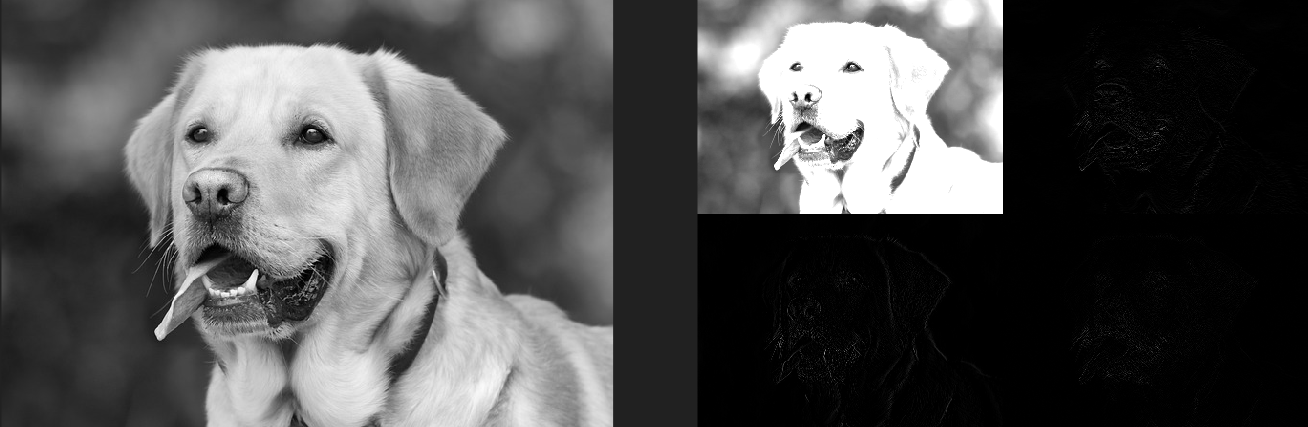
\includegraphics[width=1\textwidth]{Lv1.png}
    \caption{Hình ảnh minh họa phép biến đổi lần 1.}
\end{figure}

\noindent Biến đổi lần 2 đối với ảnh gốc là ảnh LL ta phân tích được nhiều chi tiết hơn

\begin{figure}[H]
    \centering
    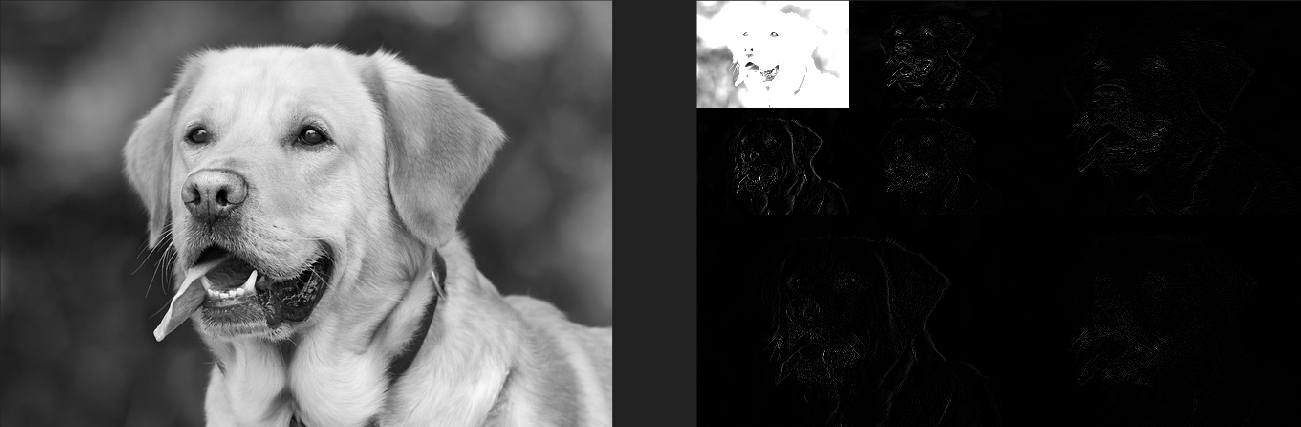
\includegraphics[width=1\textwidth]{Lv2.png}
    \caption{Hình ảnh minh họa phép biến đổi lần 2.}
\end{figure}

\subsection*{Nén không mất dữ liệu và nén mất dữ liệu}
Ý nghĩa thật sự của việc nén ảnh còn nằm ở việc tối đa hóa dữ liệu mà không làm giảm quá nhiều chất lượng ảnh.
Phương pháp này được gọi là nén mất dữ liệu. 

Một ma trận với tỷ lệ nhiều các phần tử bằng 0 được xem là thưa thớt. Đối với các ma trận ảnh, 
ma trận đã biến đổi bằng Haar Wavelet thưa hơn rất nhiều so với ma trận gốc. Hơn hết, các ma trận thưa
đơn giản hóa việc lưu trữ và truyền tải hơn ma trận ảnh gốc.

Điểm đặc biệt nhất của việc nén  mất dữ liệu này là ta có thể điều chỉnh các chi tiết ở 
vùng chi tiết cao để tạo ra nhiều phần tử 0 hơn. Để làm được điều này ta sẽ chọn một giá trị
ngưỡng $\epsilon$ và đưa tất cả hệ số chi tiết nào nhỏ hơn $\epsilon$ về 0. Sau đó ta 
thực hiện giải nén và thu được ảnh gần với ảnh gốc. Thú vị là bức ảnh thu được sau ép ngưỡng và giải 
nén gần như giống hệt ảnh gốc và hầu như rất khó nhận ra khác biệt bằng mắt thường. Phương pháp này 
được gọi là \textit{"Nén không mất dữ liệu"} nếu $\epsilon = 0$, ngược lại được gọi là 
\textit{"Nén mất dữ liệu"} nếu $\epsilon > 0$. 

Lấy ví dụ một ma trận ảnh $P$ như sau:
$$P = \begin{pmatrix}
    576 & 704 & 1152 & 1280 & 1344 & 1472 & 1536 & 1536 \\
    704 & 640 & 1156 & 1088 & 1344 & 1408 & 1536 & 1600 \\
    768 & 832 & 1216 & 1472 & 1472 & 1536 & 1600 & 1600 \\
    832 & 832 &  960 & 1344 & 1536 & 1536 & 1600 & 1536 \\
    832 & 832 &  960 & 1216 & 1536 & 1600 & 1536 & 1536 \\
    960 & 896 &  896 & 1088 & 1600 & 1600 & 1600 & 1536 \\
    768 & 768 &  832 &  832 & 1280 & 1472 & 1600 & 1600 \\
    448 & 768 &  704 &  640 & 1280 & 1408 & 1600 & 1600
\end{pmatrix}.$$
Sau phép biến đổi Haar ta thu được ma trận $T$:
$$T = \begin{pmatrix}
    1212 & -306 & -146 &  -54 &  -24 &  -68 &  -40 &   4 \\
      30 &   36 &  -90 &   -2 &    8 &  -20 &    8 &  -4 \\
     -50 &  -10 &  -20 &  -24 &    0 &   72 &  -16 & -16 \\
      82 &   38 &  -24 &   68 &   48 &  -64 &   32 &   8 \\
       8 &    8 &  -32 &   16 &  -48 &  -48 &  -16 &  16 \\
      20 &   20 &  -56 &  -16 &  -16 &   32 &  -16 & -16 \\
      -8 &    8 &  -48 &    0 &  -16 &  -16 &  -16 & -16 \\
      44 &   36 &    0 &    8 &   80 &  -16 &  -16 &   0
\end{pmatrix}.$$
Lấy ngưỡng $\epsilon = 20$, đưa tất cả hệ số chi tiết có giá trị tuyệt đối nhỏ hơn 20 về 0 ta được ma trận $D$:
$$D = \begin{pmatrix}
    1212 & -306 & -146 &  -54 &  -24 &  -68 &  -40 &   0 \\
      30 &   36 &  -90 &    0 &    0 &    0 &    0 &   0 \\
     -50 &    0 &    0 &  -24 &    0 &   72 &    0 &   0 \\
      82 &   38 &  -24 &   68 &   48 &  -64 &   32 &   0 \\
       0 &    0 &  -32 &    0 &  -48 &  -48 &    0 &   0 \\
       0 &    0 &  -56 &    0 &    0 &   32 &    0 &   0 \\
       0 &    0 &  -48 &    0 &    0 &    0 &    0 &   0 \\
      44 &   36 &    0 &    0 &   80 &    0 &    0 &   0
\end{pmatrix}.$$
Áp dụng ma trận giải nén ta thu được ảnh gốc đã qua biến đổi gọi là $R$:
$$R = \begin{pmatrix}
    582 & 726 & 1146 & 1234 & 1344 & 1424 & 1540 & 1540 \\
    742 & 694 & 1178 & 1074 & 1344 & 1424 & 1540 & 1540 \\
    706 & 754 & 1206 & 1422 & 1492 & 1572 & 1592 & 1592 \\
    818 & 866 & 1030 & 1374 & 1492 & 1572 & 1592 & 1592 \\
    856 & 808 &  956 & 1220 & 1574 & 1590 & 1554 & 1554 \\
    952 & 904 &  860 & 1124 & 1574 & 1590 & 1554 & 1554 \\
    776 & 760 &  826 &  836 & 1294 & 1438 & 1610 & 1610 \\
    456 & 760 &  668 &  676 & 1278 & 1422 & 1594 & 1594
\end{pmatrix}.$$
Ta thấy các phần tử của $R$ so với ảnh gốc $P$ có sự thay đổi gần như không đáng kể. Minh chứng
chính là sự giống nhau giữa ảnh gốc \textit{Hình 4(a)} và ảnh đã nén mất dữ liệu
\textit{Hình 4(b)}
\begin{figure}[H]
    \centering
    
\includegraphics[width=1\textwidth]{compare.png}
    \caption{Minh họa nén mất dữ liệu.}
\end{figure}



    \newpage

    \section*{Chương 2: Thuật toán và chương trình trên Matlab}
\addcontentsline{toc}{section}{Chương 2: Giải thuật nén ảnh và code Matlab}

\subsection*{1. Thuật toán nén ảnh}
Trong thực tế khi thực hiện phép nhân ma trận $B = HAH^T$ độ phức tạp thuật toán tăng lên mức 
$O(N^3)$ gây sự lãng phí tài nguyên và thời gian tính toán. Một cách tiếp cận với phép biến đổi Haar
chính là dùng thuật toán \textit{Fast Haar Wavelet Transform (FWT)} giúp giảm độ phức tạp
thuật toán xuống còn \textit{O(N)}. 

Về mặt lý thuyết ta có thể liên tục băm nhỏ một bức ảnh đến khi thành phần $LL$ chỉ còn 1 pixel duy nhất.
Ví dụ một bức ảnh độ phân giải $512 \times 512$ pixels sau 3 lần biến đổi còn lại $64 \times 64$ pixels.
Lúc này bản thân bức ảnh đã rất nhỏ, cùng với việc cắt ngưỡng quá mức có thể xóa mất những chi tiết quan trọng
khiến việc khôi phục ảnh gốc mất mát nhiều dữ liệu hơn dự tính. Do đó chúng ta có thể lựa chọn
số lần phân nhỏ ảnh gốc để đồng thời kiểm soát chất lượng bức ảnh và vẫn giữ được sự tối ưu dữ liệu.

Do đã biết bản chất phép biến đổi Haar là lấy trung bình và sai khác ta có thể giải thích thuật toán như sau:
\begin{enumerate}
    \item Khởi tạo một cell detail để lưu các ma trận chi tiết đã được phân tách.
    \item Cho vòng lặp chạy từ level 1 đến level đã chọn.
    \item Tạo các ma trận $LL$, $HL$, $LH$, $HH$ bằng một phần tư ảnh gốc.
    \item Trích xuất tập hợp $A, B, C, D$ lần lượt là ma trận các pixel ở góc trái trên cùng, góc phải trên cùng, góc trái dưới cùng, góc phải dưới cùng của mỗi khối vuông 4 pixel.
    \item Tính toán các ma trận $LL, HL, LH, HH$ theo công thức và lưu vào detail tại từng level.
    \item Gán ảnh gốc là ma trận $LL$ sau đó thực hiện tiếp biến đổi nếu chưa đi hết level đã chọn.
\end{enumerate}

Dưới đây là hàm phân giải ảnh theo thuật toán:

\begin{lstlisting}[language=Matlab]
function [LL, detailArr] = haar_decompose(img, level)
    LL = double(img);
    detailArr = cell(level, 3); 
    
    for i = 1:level
        [rows, cols] = size(LL);
        
        LL = LL(1:2*floor(rows/2), 1:2*floor(cols/2));
        
        A = LL(1:2:end, 1:2:end);
        B = LL(1:2:end, 2:2:end);
        C = LL(2:2:end, 1:2:end);
        D = LL(2:2:end, 2:2:end);
        
        LLNew = (A + B + C + D) / 2;
        HL = (A + B - C - D) / 2;
        LH = (A - B + C - D) / 2;
        HH = (A - B - C + D) / 2;

        detailArr{i, 1} = HL;
        detailArr{i, 2} = LH;
        detailArr{i, 3} = HH;
        s
        LL = LLNew; 
    end
end
\end{lstlisting}

\subsection*{2. Thuật toán cắt ngưỡng}

Giải thích thuật toán cắt ngưỡng:
\begin{enumerate}
    \item Cho một vòng lặp qua từng level, đối với từng level duyệt qua các ma trận chi tiết $HL, LH, HH$.
    \item Trong từng ma trận chi tiết thực hiện ép ngưỡng các phần tử dó giá trị tuyệt đối nhỏ hơn ngưỡng.
    \item Lưu lại ma trận chi tiết đã chỉnh sửa.
\end{enumerate}

Dưới đây là code thực hiện thuật toán trên:
\begin{lstlisting}[language=Matlab]
    for i = 1:level
        for j = 1:3
            coEff = app.detailArrAfter{i, j};
            coEff(abs(coEff) < tau) = 0;
            app.detailArrAfter{i, j} = coEff;
        end
    end

\end{lstlisting}


\subsection*{3. Thuật toán giải nén}

Giải thích thuật toán giải nén:
\begin{enumerate}
    \item Cho vòng lặp chạy từ level cao nhất trở về level thấp nhất.
    \item Tạo ma trận ảnh trống kích thước gấp đôi ma trận ảnh $LL$.
    \item Đối với mỗi level lấy thành phần $LL$ làm ảnh gốc để tái tạo các ảnh khác.
    \item Tạo ma trận $A, B, C, D$ và tính toán.
    \item Đưa từng phần tử của các ma trận $A, B, C, D$ vào các vị trí tương ứng mới.
\end{enumerate}

Dưới đây là code thực hiện thuật toán trên:
\begin{lstlisting}[language=Matlab]
    function img_recon = haar_reconstruct(LL, Details, level)
        img_recon = LL;
        for i = level:-1:1
            HL = Details{i, 1};
            LH = Details{i, 2};
            HH = Details{i, 3};

            [m, n] = size(img_recon);
            temp = zeros(2*m, 2*n);

            A = (img_recon + HL + LH + HH) / 2;
            B = (img_recon + HL - LH - HH) / 2;
            C = (img_recon - HL + LH - HH) / 2;
            D = (img_recon - HL - LH + HH) / 2;

            temp(1:2:end, 1:2:end) = A;
            temp(1:2:end, 2:2:end) = B;
            temp(2:2:end, 1:2:end) = C;
            temp(2:2:end, 2:2:end) = D;

            img_recon = temp;
        end
    end
\end{lstlisting}

\subsection*{4. Chương trình trên Matlab}

\begin{figure}[H]
    \centering
    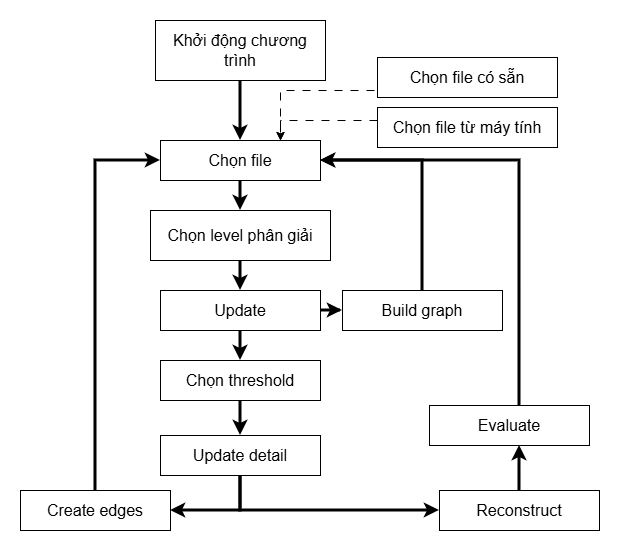
\includegraphics[width=1\textwidth]{AppFlowchart.png}
    \caption{Lưu đồ chương trình trên Matlab.}
\end{figure}

Cấu trúc chương trình có thể được diễn giải thành các bước sử dụng như sau:
\begin{enumerate}
    \item Khởi động chương trình bằng phần mềm Matlab. Chương trình được khởi động sẽ hiển thị giao diện người dùng.
    \item Nhấn chọn hình ảnh đã có sẵn hoặc nhấn \textit{Browse} để chọn ảnh bất kì trong máy tính.
    \item Sau khi chọn ảnh, hình ảnh sẽ được hiển thị. Mục \textit{Level} cũng sẽ được update để người dùng chọn cấp độ phân giải.
    \item Sau khi chọn độ phân giải người dùng nhấn \textit{Update} để tiến hành biến đổi ảnh thành các thành phần xấp xỉ và sai khác.
    \item Người dùng sau đó có thể chọn \textit{Threshold = 0} để thực hiện nén không mất dữ liệu hoặc \textit{Threshold $>$ 0} để thực hiện nén mất dữ liệu và nhấn \textit{Update detail} để cắt ngưỡng.
    \item Tiếp theo người dùng có thể chọn chức năng chính là \textit{Reconstruct} để khôi phục ảnh và nhấn \textit{Evaluate} để đánh giá mức độ khôi phục. Hoặc người dùng có thể nhấn \textit{Create edges} để thực hiện tính năng phụ là phân tích cạnh của vật thể trong ảnh.
    \item Người dùng có thể tiếp tục đánh giá phân tích ảnh bằng cách lặp lại quy trình trên.
\end{enumerate}

\noindent \textbf{Giao diện chương trình:}
\begin{figure}[H]
    \centering
    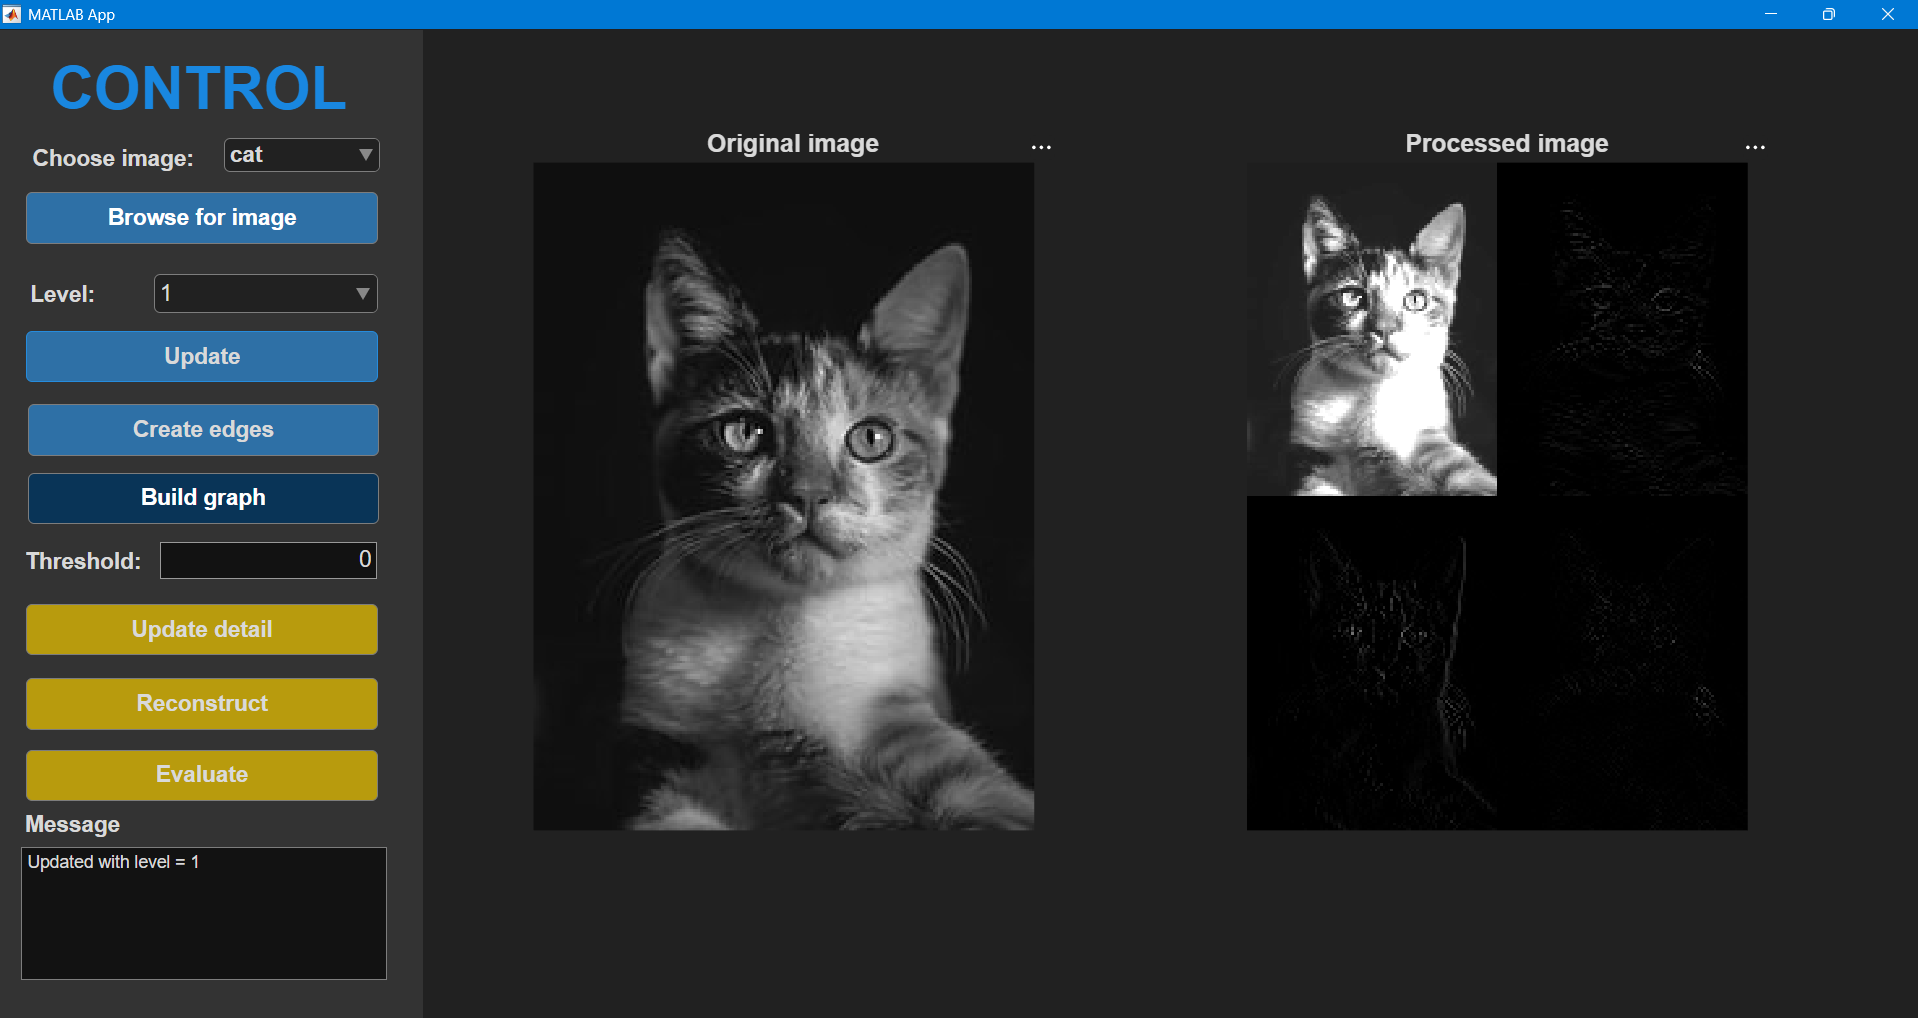
\includegraphics[width=1\textwidth]{App_UI.png}
    \caption{Giao diện chương trình trên Matlab.}
\end{figure}

    \newpage

    \section*{Chương 3: Kết quả và đánh giá}
\addcontentsline{toc}{section}{Chương 3: Kết quả và đánh giá}

\subsection*{1. Phương pháp đánh giá}
\subsubsection*{1.1. Tỷ lệ triệt tiêu dữ liệu (Sparsity)}
\noindent Thông số Sparsity thể hiện tỷ lệ phần tử chi tiết trong ảnh sau khi cắt ngưỡng bị triệt tiêu trên tổng số phần tử của bức ảnh.
$$Sparsity = \frac{N_{zero}}{N_{total}} \times 100\%$$
Trong đó:
\begin{itemize}
    \item $N_{zero}$: Số lượng các phần tử bằng 0 của ảnh sau khi nén.
    \item $N_{total}$: Tổng số lượng điểm ảnh của bức ảnh gốc.
\end{itemize}
\noindent Về mặt ý nghĩa, Sparsity càng cao tức là số lượng phần tử chi tiết bị triệt tiêu trong quá trình nén ảnh càng nhiều,
giúp dung lượng file giảm đi tương đương. Tuy nhiên Sparsity quá cao có thể làm mất chi tiết trong ảnh mặc cho đã tiết kiệm được dung lượng.


\subsubsection*{1.2. Sai số toàn phương trung bình (Mean Squared Eror - MSE)}
\noindent MSE là trung bình bình phương sự chênh lệch từng điểm ảnh giữa ảnh gốc và ảnh đã nén.
$$MSE = \frac{1}{m.n} \sum_{i=1}^{m} \sum_{j=1}^{n} \left[ I(i,j)-K(i,j) \right]^2$$
Trong đó:
\begin{itemize}
    \item $m,n$: Là kích thước của ảnh.
    \item $I$: Ma trận ảnh gốc.
    \item $K$: Ma trận ảnh đã khôi phục.
\end{itemize}
\noindent Nếu $MSE=0$ nghĩa là không có sự chênh lệch nào, ngược lại $MSE$ càng cao càng có sự chênh lệch giữa ảnh gốc và ảnh đã giải nén.


\subsubsection*{1.3. Tỷ số tín hiệu cực đại trên nhiễu (Peak Signal to Noise Ratio - PSNR)}
\noindent Thông số PSNR (đơn vị Decibel - dB) là thông số quan trọng cho biết trực tiếp chất lượng ảnh sau giải nén so với ảnh gốc.
Thông số dựa trên tỉ lệ giữa bình phương phần tử có độ sáng lớn nhất chia cho MSE và được ép tỷ lệ qua hàm logarith.
$$PSNR=10.log_{10} \left( \frac{MAX_I^2}{MSE} \right)$$
Trong đó:
\begin{itemize}
    \item $MAX_I$: Giá trị của điểm ảnh sáng nhất.
    \item $MSE$: Sai số toàn phương trung bình.
\end{itemize}
\noindent PSNR càng cao (lý tưởng từ 30 dB trở lên) tương đương với việc bức ảnh được nén và khôi phục rất tốt, mắt người khó phân biệt
được sự khác biệt với ảnh gốc. Ngược lại PSNR càng thấp, ảnh càng vỡ và mất chi tiết.

\subsubsection*{1.4. Tỷ lệ nén (Compression Ratio)}
Tỷ lệ nén thể hiện tỷ lệ tối ưu về mặt lưu trữ dữ liệu của ảnh nén so với ảnh chưa nén. Ví dụ tỷ lệ nén là $1:4$ tương đương ảnh đã nén chỉ chiếm lượng lưu trữ bằng một phần tư ban đầu.
$$Compression Ratio = \frac{N_{non-zero}}{N_{total}}$$
Trong đó:
\begin{itemize}
    \item $N_{non-zero}$: Số lượng các phần tử khác 0 của ảnh sau khi nén.
    \item $N_{total}$: Tổng số lượng điểm ảnh của bức ảnh gốc.
\end{itemize}

\subsection*{2. Thực hiện đánh giá}
\noindent Thực hiện đánh giá ảnh gốc là ảnh chú chó trong hình sau:
\begin{figure}[H]
    \centering
    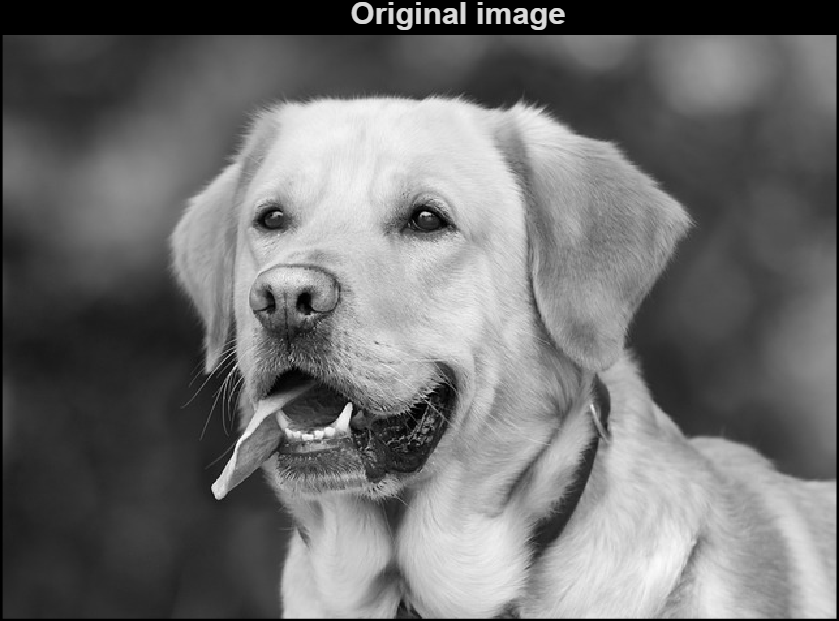
\includegraphics[width=1\textwidth]{dog.png}
    \caption{Ảnh gốc chú chó.}
\end{figure}
\noindent Với các thông số:
\begin{itemize}
    \item $Level=2$.
    \item $Threshold=50$
\end{itemize}

\noindent Thực hiện tái tạo ta thu được ảnh chú chó:
\begin{figure}[H]
    \centering
    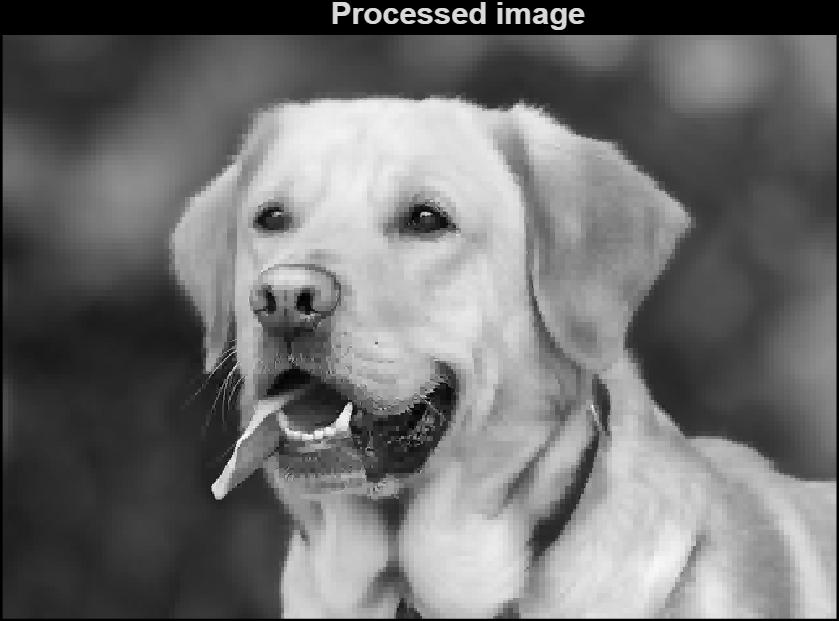
\includegraphics[width=1\textwidth]{Dog_evaluate.png}
    \caption{Ảnh chú chó đã khôi phục.}
\end{figure}
\noindent Kết quả phân tích ảnh thu được như sau:
\begin{itemize}
    \item $MSE=46.12$
    \item $PSNR=31.49 dB$
    \item $Sparsity=93.11\%$
    \item $Compression Ratio = 1:14.50$
\end{itemize}
\noindent Với mức ngưỡng 50 được cho là khá cao, tỷ lệ nén lúc này cho thấy ảnh chú cho khi nén giúp tối ưu lưu trữ đến hơn 14 lần. Để ý ta thấy phần hậu cảnh
được chụp với hiệu ứng bokeh, tức là hậu cảnh đã được làm mờ, tương đương đến sự khác biệt về chi tiết trong hậu cảnh là không đáng kể. Do đó mặc
dù chỉ số PSNR không quá thấp nhưng ta vẫn thấy được sự vỡ ảnh ở chú chó do phần lớn sự triệt tiêu xảy ra trên chú chó này.

\noindent Ở lần thử tiếp theo hãy thử hạ thấp mức ngưỡng xuống còn 20 và xem điều gì sẽ xảy ra:
\begin{figure}[H]
    \centering
    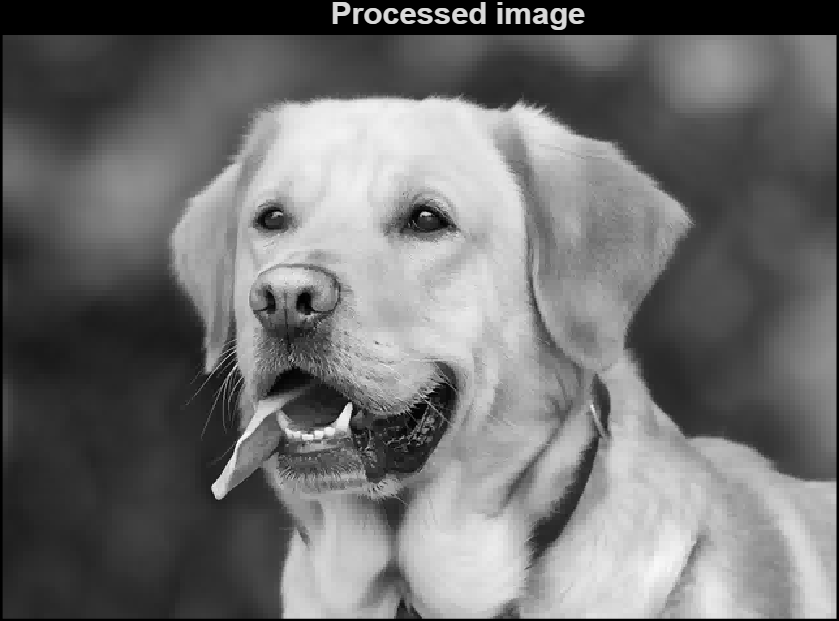
\includegraphics[width=1\textwidth]{Dog_evaluate2.png}
    \caption{Ảnh chú chó đã khôi phục lần thử 2.}
\end{figure}
\noindent Kết quả phân tích ảnh thu được như sau:
\begin{itemize}
    \item $MSE=18.47$
    \item $PSNR=35.47 dB$
    \item $Sparsity=90.15\%$
    \item $Compression Ratio = 1:10.15$
\end{itemize}
\noindent Các chi tiết trên khuôn mặt chú chó lúc này gần như không thể phân biệt so với ảnh gốc, tương ứng với PSNR đã tăng đến 35.47 đánh đổi bằng việc
dung lượng lưu trữ tăng lên nhưng vẫn giữ tỷ lệ đáng kể ít hơn một phần mười so với ảnh gốc.
    \newpage

    \section*{Chương 4: Tổng kết}
\addcontentsline{toc}{section}{Chương 4: Tổng kết}

\subsection*{1. Ưu điểm và kết quả đạt được}
Qua quá trình nghiên cứu và thực hiện đề tài, nhóm đã hoàn thành các mục tiêu đã đặt ra và rút ra một số ưu điểm như sau:
\begin{itemize}
    \item Hiểu rõ hơn bản chất lý thuyết đằng sau phép biến đổi Haar. Củng cố các kiến thức Đại số tuyến tính đã được học.
    \item Chương trình được xây dựng với giao diện rõ ràng, giúp trực quan hóa quá các quá trình nén ảnh bằng hình ảnh, thông số và đồ thị.
    \item Nhóm đã phân tích được các phương pháp và thông số đánh giá mức độ nén của một bức ảnh. Ngoài ra còn có các nhận xét sâu hơn về tính ứng dụng của phép biến đổi Haar Wavelet trong xử lý ảnh.
    \item Quá trình làm việc chung đã giúp các thành viên rèn luyện tính kỷ luật, nâng cao kỹ năng giao tiếp, giải quyết vấn đề và tinh thần trách nhiệm trong làm việc nhóm.
\end{itemize}
\subsection*{2. Nhược điểm và hướng phát triển}
Bên cạnh những kết quả tích cực, đề tài vẫn còn một số điểm giới hạn có thể tiếp tục phát triển trong tương lai:
\begin{itemize}
    \item Thuật toán và chương trình hiện tại chỉ có thể nén ảnh tĩnh và ảnh xám. Đối với ảnh động và ảnh màu cần nhiều kỹ thuật và lý thuyết hơn. 
    Tuy vậy với nền tảng sử dụng phép biến đổi Haar Wavelet, nhóm có khả năng để thực hiện các phép biến đổi phức tạp hơn cho nhiều đối tượng hơn trong tương lai.
    \item Các thông số đánh giá được sử dụng đôi khi không thể hiện chính xác chất lượng ảnh đối với ảnh có nhiều thông tin phức tạp như hiệu ứng hậu cảnh bokeh. Hướng phát triển là 
    học hỏi thêm các thông số đánh giá nâng cao để thực hiện phân tích chính xác chất lượng ảnh.
\end{itemize}
    \newpage

    \input{Ending.tex} 
    \newpage

    \section*{TÀI LIỆU THAM KHẢO}
\addcontentsline{toc}{section}{TÀI LIỆU THAM KHẢO}

\begin{thebibliography}{99}

\bibitem{dangvanvinh} 
Đ. V. Vinh, \textit{Giáo trình đại số tuyến tính}. Bộ môn Toán Ứng dụng, Khoa Khoa học Ứng dụng, Trường Đại học Bách Khoa - ĐHQG-HCM.

\bibitem{anton1994} 
H. Anton and C. Rorres, \textit{Elementary Linear Algebra: Applications Version}, 7th ed. New York, NY, USA: John Wiley \& Sons, Inc., 1994.

\bibitem{meyer2000} 
C. D. Meyer, \textit{Matrix Analysis and Applied Linear Algebra}. Philadelphia, PA, USA: SIAM, 2000.

\bibitem{kolman1997} 
B. Kolman, \textit{Introductory Linear Algebra with Applications}. New Jersey: Prentice Hall, Inc., 1997.

\bibitem{sethi_ijarcs} 
N. Sethi, R. Krishna, and R. P. Arora, ``Image Compression Using Haar Wavelet Transform,'' \textit{International Journal of Advanced Research in Computer Science}.


\bibitem{roberts_lossless} 
E. Roberts, ``Lossless Compression: An Overview,'' Stanford University. [Online]. Available: \url{https://cs.stanford.edu/people/eroberts/courses/soco/projects/data-compression/lossless/index.html}

\bibitem{sciencedirect_lossless} 
``Lossless Compression,'' ScienceDirect, Elsevier. [Online]. Available: \url{https://www.sciencedirect.com/topics/engineering/lossless-compression}

\bibitem{singh2016} 
M. Singh, S. Kumar, S. Chouhan, and M. Shrivastava, ``Various Image Compression Techniques: Lossy and Lossless,'' \textit{International Journal of Computer Applications}, vol. 142, pp. 23--26, 2016, doi: 10.5120/ijca2016909829.

\bibitem{akansu2001} 
A. N. Akansu and R. A. Haddad, ``Chapter 2 - Orthogonal Transforms,'' in \textit{Multiresolution Signal Decomposition}, 2nd ed., A. N. Akansu and R. A. Haddad, Eds. Academic Press, 2001, pp. 11--111. doi: 10.1016/B978-012047141-6/50002-1.

\bibitem{bull2021} 
D. R. Bull and F. Zhang, ``Chapter 5 - Transforms for image and video coding,'' in \textit{Intelligent Image and Video Compression}, 2nd ed., D. R. Bull and F. Zhang, Eds. Academic Press, 2021, pp. 143--182. doi: 10.1016/B978-0-12-820353-8.00014-1.

\bibitem{porwik2004} 
P. Porwik and A. Lisowska, ``The Haar-wavelet transform in digital image processing: its status and achievements,'' \textit{Machine Graphics and Vision}, vol. 13, 2004.
\end{thebibliography}
    \newpage

\end{document}